\documentclass{article}
\usepackage{blindtext}
\usepackage[a4paper, total={7in, 10in}]{geometry}
\usepackage{tikz}
\usetikzlibrary{quotes}

\newcommand{\FixedLengthArrow}{2,0}

\title{Formális nyelvek szóbeli tételek kidolgozása}
\begin{document}
    \pagenumbering{gobble}
    \maketitle
    \newpage
    \pagenumbering{arabic}
    
    \section{A környezetfüggetlen nyelvtan definíciója, a levezetés és a nyelvtan által generált nyelv fogalma. A reguláris nyelvtan és nyelv definíciója}
    \subsection{környezetfüggetlen nyelvtan}
    \setlength{\parskip}{ 4mm minus 3mm}
    
    \begin{itemize}
        \item N egy ábécé, nemterminális ábécé
        \item $ \Sigma $ egy ábécé, a terminális (befejező, végső) ábécé, amire N $ \bigcap \Sigma $ = $ \emptyset $
        \item S $ \in $ N a kezdőszimbólum (vagy start szimbólum)
        \item P pedig A $ \rightarrow \alpha $  alakú ún. átírási szabályok véges halmaza, ahol A $ \in $ N és $ \alpha \in $ (N $ \bigcup \Sigma $ )*
    \end{itemize}

    $ \rightarrow $ Példa:
    \hspace{\parindent}  \[G_1 =(\{S\},\{a,b\},\{S \rightarrow aSb,S \rightarrow \epsilon\},S)\]

    \subsection{Közvetlen levezetés (deriváció)}

    Tetszőleges $ \gamma $, $ \beta \in $ (N $ \bigcup \Sigma $)* esetén $ \gamma \Rightarrow _G \beta $,
    ha van olyan A $ \rightarrow \alpha \in $ P szabály és vannak olyan $ \alpha^{'}, \beta^{'} \in (N \bigcup \Sigma)^* $ szavak,
    amelyekre fennállnak, hogy $ \gamma = \alpha^{'}A\beta^{'} $, $ \beta = \alpha^{'}\alpha\beta^{'} $ 

    \newblock
    \newline
    $ \rightarrow $ Példa:
    \[G_1 = (\{S\}, \{a, b\}, \{S \rightarrow aSb, S \rightarrow \epsilon\}, S)\]
    \begin{center}
        $ bSa \Rightarrow _{G_1} baSba $ az $ S \rightarrow aSb $ szabállyal\\
        $ baaSa \Rightarrow _{G_1} baaa $ az $ S \rightarrow \epsilon $ szabállyal
    \end{center}

    \subsection{Levezetések}

    \begin{itemize}
        \item $ \gamma \Rightarrow _G \beta $: egy lépés (= a közvetlen levezetés)
        \item $ \gamma \Rightarrow _G^n \beta $: n $ \ge $ 0 lépés ($ \gamma \Rightarrow _G^0 \beta \Leftrightarrow \gamma = \beta $)
        \item $ \gamma \Rightarrow _G^+ \beta $: legalább egy lépés
        \item $ \gamma \Rightarrow _G^* \beta $: valamennyi (esetleg 0) lépés
        \item A G = (N, $ \Sigma $ , P, S) környezetfüggetlen nyelvtan által generált nyelv: L(G) = \{ $ w \in \Sigma ^* | S \Rightarrow _G^* w $\}\\
        $ \rightarrow $ Az $ w \in \Sigma ^* $ feltétel miatt w-ben nincsenek nemterminálisok, tegát nem lehet belőle "tovább lépni". \\$ \rightarrow $ pl.
        $ L(G_1) = \{ a^n b^n | n \ge 0 \} $
    \end{itemize}

    *A nyelv és a nyelvtan két különböző fogalom. Egy nyelv szavak egy (véges vagy végtelen) halmaza, míg egy nyelvtan egy olyan végesen specifikált (adott) eszköz, amellyel nyelvet lehet generálni.\\
    L(G) = L($ G^{'} $)

    \subsection{környezetfüggetlen nyelvek}

    Egy L nyelvet környezetfüggetlen nyelvnek hívunk, ha van olyan G környezetfüggetlen nyelvtan, melyre L = L(G). Az összes környezetfüggetlen nyelvek halmazát CF-fel jelöljük.

    \subsection{Reguláris nyelvtanok}
    

    Egy G = (N, $ \Sigma $, P, S) nyelvtan reguláris (vagy jobblineáris), ha P-ben minden szabály A $ \rightarrow $ xB vagy A $ \rightarrow $ x alakú.
    Reguláris nyelvtan esetén minden levezetés \\ \newline
    \indent $ A _1 \Rightarrow x_1 x_2 A_3 \Rightarrow ... \Rightarrow x_1 x_2 ... x_n A_{n+1} $ \\ \newline
    alakú, ahol az alkalmazott szabályok \\ \newline
    \indent $ A_1 \rightarrow x_1 A_2, A_2 \rightarrow x_2 A_3, ..., A_n \rightarrow x_n A_{n+1} $ \\

    Levezetést csak $ A \rightarrow x $ alakú szabállyal fejezhetünk be. Ugyanez érvényes minden olyan szóra, amelyet az S kezdőszimbólumból vezetünk le. \\ \newline
    \indent Definíció szerint minden reguláris nyelvtan környezetfüggetlen, mert az $ A \rightarrow xB $ szabályok esetén $ xB \in (N \bigcup \Sigma)^* $ és az $ A \rightarrow x $ szabályok esetén $ x \in (N \bigcup \Sigma)^* $.
    \newline \newline
    $ \rightarrow $ Példa: G$_3 \Rightarrow S \rightarrow aS | bS | \epsilon $ \\ \newline
    \indent \indent L(G$_3$) = $ \Sigma ^* $ és $ \Sigma $ = \{a, b\} \\
    \indent \indent abb levezetése: $ S \Rightarrow aS \Rightarrow abS \Rightarrow abbs \Rightarrow abb $ \\
    \indent \indent Derivációt csak az $ S \rightarrow \epsilon $ szabállyal tudjuk befejezni.

    \subsection{Reguláris nyelvek}

    Egy L nyelvet reguláris nyelvnek hívunk, ha van olyan G reguláris nyelvtan, melyre L = L(G). Az összes reguláris nyelvek halmazát REQ-gel jelöljük. Például az $ \emptyset $, az \{ $a^n b^m | n, m \ge 0 $\} nyelv, és minden véges nyelv reguláris. \\
    REQ $ \subseteq $ CF

    \newpage
    \section{Véges automata fogalma, felismert nyelv, kiterjesztések és ezek ekvivalenciája}

    \subsection{Véges automaták fogalma}

    \subsubsection{Determinisztikus automata}

    Az M = (Q, $ \Sigma, \beta, q_0, F $) rendszert determinisztikus automatának nevezzük, ahol:
    \begin{itemize}
        \item Q - Egy nem üres, véges halmaz, az állapotok halmaza
        \item $ \Sigma $ - Egy ábécé, az input ábécé
        \item $ q_0 \in Q $ - Kezdőállapot
        \item $ F \subseteq Q $ - A végállapotok halmaza 
        \item $ \beta: Q \ x \ \Sigma \rightarrow Q $ - Egy leképezés, az átmenetfüggvény
    \end{itemize}
    Gráfként: \\ \newline

    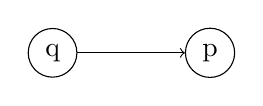
\begin{tikzpicture}[main/.style = {draw, circle}, node distance=4cm]
        \node[main] at (0, 0) (1) {q};
        \node[main] at (2, 0) (2) {p};
        \draw[->, to path={-- (\tikztotarget)}] (1) edge (2.west);
    \end{tikzpicture} \\ \newline

    $ \rightarrow $ Példa: M$_3$ = (Q, $ \Sigma, \beta, q_0, F $) \\
    \indent Q = ($ q_0, q_1, q_2$)\hspace{1cm} $ \beta(q_0, a) = q_1, \beta(q_0, b) = q_0 $ \\
    \indent $ \Sigma = {a, b} $ \hspace{2cm} $ \beta(q_1, a) = q_2, \beta(q_1, b) = q_1 $ \\
    \indent F = { $q_0$} \hspace{2.02cm} $ \beta(q_2, a) = q_0, \beta(q_2, b) = q_2 $ \\ \newline

    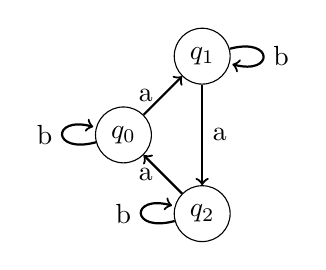
\begin{tikzpicture}[main/.style = {draw, circle} ]
        \node at (0, 1) [main] (1) {$q_0$};
        \node at (1, 2) [main] (2) {$q_1$};
        \node at (1, 0) [main] (3) {$q_2$};

        \path[->, draw, thick]
        (1) edge [loop left] node[name=q0b]  {b} (1)
        (1) edge node[name=q0a] [loop left] {a} (2)
        (2) edge [loop right] node [name=q1b] {b} (2)
        (2) edge node[name=q1a] [loop right] {a} (3)
        (3) edge [loop left] node [name=q2b] {b} (3)
        (3) edge node [name=q2a] [loop left] {a} (1);
    \end{tikzpicture}

    \noindent M konfigurációinak halmaza: C = Qx$ \Sigma^* $ \\ 
    A (q, $a_1...a_n$) konfiguráció azt jelenti, hogy M a q állapotbanvan és az $a_1...a_n$ szót kapja inputként. \\ \newline
    Átmeneti reláció:
    \begin{itemize}
        \item (q, w) , ($ q^{'}, w^{'}$) $ \in $ C esetén (q, w) $ \vdash_M $ ($ q^{'}, w^{'}$), ha w = aw$^{'}$, valamely $ a \in \Sigma $-ra és $ \beta(q, a) = q^{'} $
        \item (q, w) $ \vdash_M (q^{'}, w^{'}) $, egy lépés
        \item (q, w) $ \vdash_M^n (q^{'}, w^{'}) $, n $ \ge $ 0 lépés
        \item (q, w) $ \vdash_M^+ (q^{'}, w^{'}) $, legalább 1 lépés
        \item (q, w) $ \vdash_M^* (q^{'}, w^{'}) $, valamennyi (esetleg 0) lépés
    \end{itemize}

    \noindent Az M = (Q, $ \Sigma, \beta, q_0$, F) automata által felismert nyelven az \\
    L(M) = \{$ w \in \Sigma^* | (q_0, w) \vdash_M^* (q, \epsilon) $ és $ q \in F $\}

    \subsubsection{Nemdeterminisztikus automata}
    Az M = (Q, $ \Sigma, \beta, q_0, F $) rendszert Nemdeterminisztikus automatának nevezzük, ahol:
    \begin{itemize}
        \item Q - egy nem üres, véges halmaz, az állapotok halmaza
        \item $ \Sigma $ - egy ábécé, az input ábécé
        \item $ q_0 \in Q $ - a kezdőállapot
        \item $ F \subseteq Q $ - a végállapotok halmaza
        \item $ \beta: Qx\Sigma \rightarrow \mathcal{P}(Q) $ egy leképezés, az átmenetfüggvény
    \end{itemize}
    \noindent Nemdeterminisztikus: egy input szimbólum hatására egy állapotból több állapotba is átmehet. \\
    $ \rightarrow $ Példa: $ \beta(q, a) = \{q_1,...,q_n\} $

    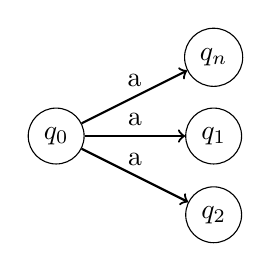
\begin{tikzpicture}[main/.style = {draw, circle} ]
        \node at (0, 1) [main] (1) {$q_0$};
        \node at (2, 1) [main] (2) {$q_1$};
        \node at (2, 0) [main] (3) {$q_2$};
        \node at (2, 2) [main] (4) {$q_n$};

        \path[->, draw, thick]
        (1) edge node[name=q1a] [loop above] {a} (2)
        (1) edge node[name=q2a] [loop above] {a} (3)
        (1) edge node[name=q3a] [loop above] {a} (4);
        
    \end{tikzpicture}

    \noindent Az átmeneti reláció és a felismert nyelv nemdeterminisztikus autmoatákra: \\
    \indent (q, w), ($q^{'}, w^{'}$) $ \in $ C esetén (q, w) $ \vdash_M (q^{'}, w^{'})$, ha w = a$w^{'}$, valamely $ a \in \Sigma $-ra  és $ q^{'} \in \beta(q, a) $
    \\ \newline
    \noindent Az M = (Q, $ \Sigma,  \beta, q_0, F $) automata által felismert nyelven az \\
    \indent L(M) = \{$ w \in \Sigma^* | (q_0, w) \vdash_M^* (q, \epsilon ) $ valamely $ q \in F $ -re \} nyelvet értjük. \\ \newline
    \indent Az M = (Q, $ \Sigma, \beta, q_0, F $) nemdeterminisztikus automata teljesen definiált, ha minden $ q \in Q$ és $ a \in \Sigma $ esetén $ \beta(q, a) $ legalább egy elemű \\ \newline
    

\end{document}